\chapter[Data and Methods]{Data and Methods}

This chapter starts with a small section on the research area. \ref{area}
Then, per research question a section is dedicated, describing its data, pre-preprocessing steps and the analysis. The critical walkability factors will be explored in section \ref{rq1} through literature studies and interviews. Also a short sub-section on the average walking speed of elderly is present. 
Section \ref{rq2a} shows the data collection and pre-processing steps for the analysis of existing geo-data. The GBKA an the AHN are used.
In section \ref{rq2b} the data collection and pre-processing steps for the collection of our own geo data, with GPS devices and an accelerometer. Eventually, the steps for analysing this data is explained in the last part of this section.
The methods for combining the existing geo-data with the own collected data is explained in section \ref{rq2c}. With a Change Point detection algorithm, changes in the time series of the rollator walks are found, and plotted on the map to compare it to other data sources. 
\clearpage
\section{Study area}\label{area}
This project in conducted for the project MeetRollator in the scope of the recently founded Amsterdam Institute For Advanced Metropolitan Solutions (AMS). The study area of AMS in Amsterdam, see left figure ~\ref{kaart} for the location. The Amsterdam Municipality contributed with data that covers the centre area of Amsterdam, indicated with the red square in the right figure ~\ref{kaart}. 
The literature study, interviews, AHN study will be mostly focussed on this area. The more general measurements were taken in Wageningen due to a more conventional location and travelling circumstances for the conducting researcher. See figure ~\ref{tracks} from chapter 3.5. 

\begin{figure}[h]
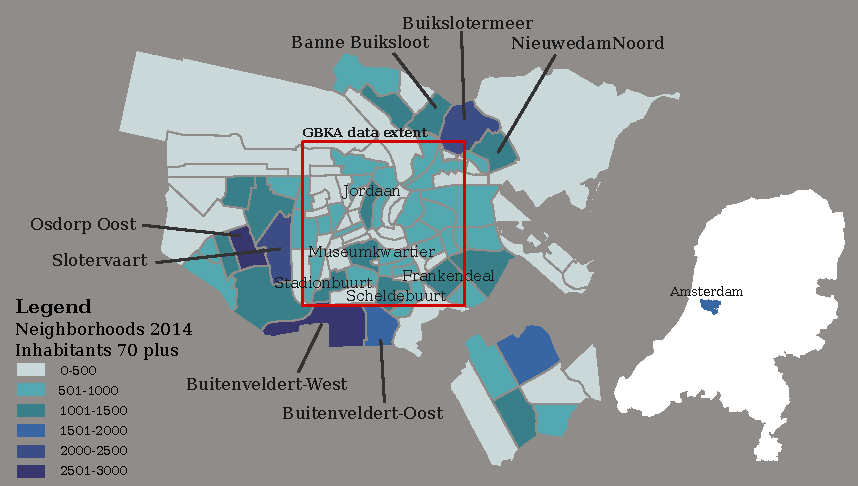
\includegraphics[width=\textwidth]{img/M1_StudyArea.pdf}
\centering
\caption{Study area Amsterdam, The Netherlands\label{kaart}}
\end{figure}

There is no exact information on the amount of elderly using a rollator in Amsterdam or where they live. There for the CBS statistics of 2013 were used to detect the neighbourhoods were the most elderly above 70 live. In figure ~\ref{kaart} can be seen that in the centre the most elderly live in the Jordaan. In the whole of Amsterdam the most elderly can be found in the South West and North.  